\chapter{模板使用说明}

{\Large\heiti 本文档是上海科技大学本硕博学位论文模板的简要使用说明。}

\section{模板组成}
\subsection{文档最主要的控制文件}
\begin{verbatim}
        1. ShanghaiTechThesis.cls 文件:模板文件类,格式控制文件
        2. ShanghaiTechThesis.tex 文件:主控文件,控制模板内容的流程
\end{verbatim}

\subsection{文件夹} 
\begin{verbatim}
        1. declare 文件夹:放置编写声明类的文件
        2. frontmatter 文件夹:放置目录之前的摘要符号等论文的说明类文档
        3. mainmatter 文件夹:用于编写论文章各个章节和各个附录,之后再 include 到 tex 主文件
        4. backmatter 文件夹:放置各种说明性文件,如致谢,公开作品,个人简历等
        5. bibliography 文件夹:用于放置文献资料的 .bib 文件
        7. picture 文件夹:用于存放文章中插入的图片
        8. logo 文件夹:用于放置学校校徽图片等的文件夹
\end{verbatim}

\section{.tex 文件基本结构}
{\heiti .tex 文件基本结构是对论文的基本顺序的控制}
\begin{verbatim}
        1. ducumentclas{ShanghaiTechThesis}:调用 ShanghaiTechThesis.cls 文档类
        2. 导言区:填写标题页相关信息
# 以下是论文结构\begin{document}
        3. \maketitle \makeentitle :编制标题页
        4. \declarerriginal \declareauthorization 原创性声明和授权书
# \frontmatter 以上不计页码,以下开始有罗马数字页码
        5. 依次导入中英文摘要、文档目录、插图目录、表格目录和算法目录
# \mainmatter 开始导入正式章节,页码转变为阿拉伯数字
        6. include{mainmatter/chapter num}
# \appendix 开始导入附录章节
        7. include{mainmatter/appendix num}
# \backmatter 
        8. 导入 bibliography 文件夹里的参考文献
        9. include{frontmatter/filename} :导入致谢、发表论文、申请专利、参与项目、简历等
\end{verbatim}
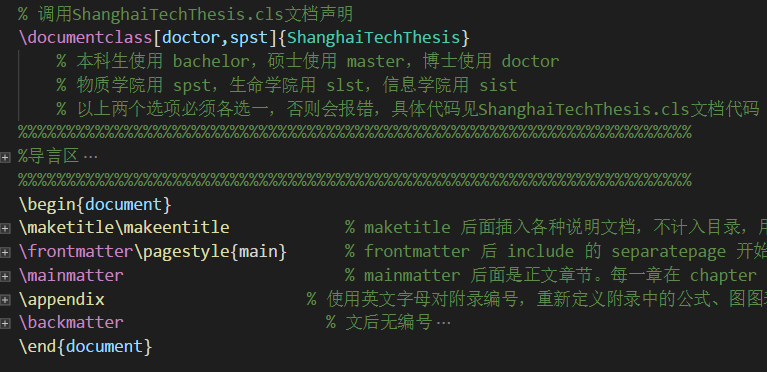
\includegraphics{picture/tex.png}
\section{.cls 文档类的基本结构}
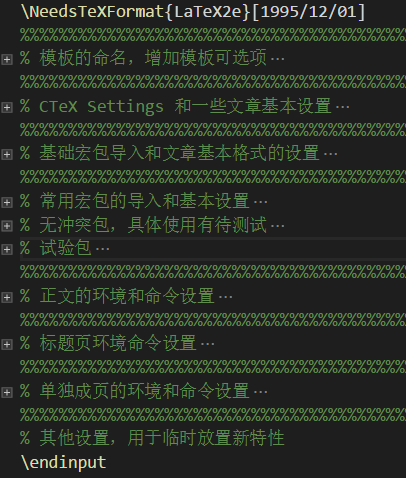
\includegraphics{picture/cls.png}
\section{模板使用方法}
\begin{verbatim}
        1. \documentclass[master,spst]{ShanghaiTechThesis}
        % 本科生使用 bachelor,硕士使用 master,博士使用 doctor
        % 物质学院用 spst,生命学院用 slst,信息学院用 sist
        % 以上两个选项必须各选一,否则会报错,具体见 ShanghaiTechThesis.cls 文档代码

        2. 在 mainmatter 文件夹里按顺序编写论文,如需导入新的宏包或设置新命令,在 .cls 文件设置
        文件引用的文献在 bibliography 文件夹里的 .bib 文件里编译
        文件引用的图片放在 picture 里,用 \includegraphics[]{picture/pic name} 调用
\end{verbatim}